\documentclass[conference]{IEEEtran}
\IEEEoverridecommandlockouts
% The preceding line is only needed to identify funding in the first footnote. If that is unneeded, please comment it out.
\usepackage{cite}
\usepackage{amsmath,amssymb,amsfonts}
\usepackage{algorithmic}
\usepackage{graphicx}
\usepackage{textcomp}
\usepackage{xcolor}
\usepackage{url}
\usepackage{hyperref}
\def\BibTeX{{\rm B\kern-.05em{\sc i\kern-.025em b}\kern-.08em
    T\kern-.1667em\lower.7ex\hbox{E}\kern-.125emX}}
\begin{document}

\title{CS6888 Software Analysis and its Applications \\ HW1\\
% {\footnotesize \textsuperscript{*}Note: Sub-titles are not captured in Xplore and
% should not be used}
% \thanks{Identify applicable funding agency here. If none, delete this.}
}

\author{\IEEEauthorblockN{Sravanth Chowdary Potluri}
\IEEEauthorblockA{und5uv@virginia.edu}
\textit{University Of Virginia}\\
% City, Country \\
% email address or ORCID}
% \and
% \IEEEauthorblockN{2\textsuperscript{nd} Given Name Surname}
% \IEEEauthorblockA{\textit{dept. name of organization (of Aff.)} \\
% \textit{name of organization (of Aff.)}\\
% City, Country \\
% email address or ORCID}
% \and
% \IEEEauthorblockN{3\textsuperscript{rd} Given Name Surname}
% \IEEEauthorblockA{\textit{dept. name of organization (of Aff.)} \\
% \textit{name of organization (of Aff.)}\\
% City, Country \\
% email address or ORCID}
% \and
% \IEEEauthorblockN{4\textsuperscript{th} Given Name Surname}
% \IEEEauthorblockA{\textit{dept. name of organization (of Aff.)} \\
% \textit{name of organization (of Aff.)}\\
% City, Country \\
% email address or ORCID
% \and
% \IEEEauthorblockN{5\textsuperscript{th} Given Name Surname}
% \IEEEauthorblockA{\textit{dept. name of organization (of Aff.)} \\
% \textit{name of organization (of Aff.)}\\
% City, Country \\
% email address or ORCID}
% \and
% \IEEEauthorblockN{6\textsuperscript{th} Given Name Surname}
% \IEEEauthorblockA{\textit{dept. name of organization (of Aff.)} \\
% \textit{name of organization (of Aff.)}\\
% City, Country \\
% email address or ORCID}
}

\maketitle

% \begin{abstract}
% This document is a model and instructions for \LaTeX.
% This and the IEEEtran.cls file define the components of your paper [title, text, heads, etc.]. *CRITICAL: Do Not Use Symbols, Special Characters, Footnotes, 
% or Math in Paper Title or Abstract.
% \end{abstract}

% \begin{IEEEkeywords}
% component, formatting, style, styling, insert
% \end{IEEEkeywords}

\section{Strategies Used to Increase AFL Coverage}

To systematically increase the coverage generated by the AFL fuzzer, a variety of strategies were explored through 16 different checkpoints. These checkpoints can be accessed in the 'Checkpoints' Directory of the HW1 directory in the repository.

\subsection{Checkpoint Progression and Observations}

\begin{enumerate}
    \item 	\textbf{Baseline Attempt}: The fuzzer was initially run with just the provided `hello.c` seed. However, AFL was unable to run properly due to insufficient memory allocation, as the required memory exceeded the 50 MB default. Despite this, a coverage of 34.5\% was achieved due to compiler execution errors being triggered. This approach was deemed unsustainable since the compiler was unable to properly execute test cases.
    
    \item 	\textbf{Increasing Memory Allocation}: The memory limit was increased to 500 MB and the fuzzer was run again with only `hello.c`. The coverage dropped to 18\%, indicating that the original coverage had been inflated due to error handling rather than actual program execution.
    
    \item 	\textbf{Increasing Execution Time}: The execution time was increased from 10 minutes to 25 minutes to allow AFL to explore more paths. However, the coverage only marginally improved to 18.3\%, suggesting that time alone was not a sufficient strategy for increasing coverage.
 
    \item 	\textbf{Expanding the Seed Corpus}: Multiple seed programs were added, each designed to test various functionalities of the compiler. This significantly increased coverage to 51.8\%, confirming that a more diverse seed pool was an effective approach.
    
    \item 	\textbf{Modifying Compiler Options}: Different compiler options were tested in the run string to force the compiler to execute more code paths. This increased coverage to 53.4\%.
    
    \item 	\textbf{Adding Assembly-Based Seed Programs}: Since certain parts of the compiler related to ASM processing were not covered, assembly test files were introduced. This improved coverage further to 55.3\%.
    
    \item 	\textbf{Further Expanding the Seed Corpus}: More C and assembly seed programs were added to explore niche functionalities. This increased coverage to 56.7\%, although diminishing returns were observed.
    
    \item 	\textbf{Using an AFL Dictionary}: A dictionary of C language keywords was used to guide AFL's mutations. This resulted in a slight increase to 56.9\%, demonstrating limited but measurable improvement.
    
    \item 	\textbf{Reducing Memory Allocation}: The memory limit was reduced from 500 MB to 300 MB to prevent high-memory test cases from hogging CPU Time. However, this caused a decrease in coverage to 56.6\%, leading to a reversal of this change.
    
    \item 	\textbf{Using the -run Compiler Option}: The `-run` flag was added to the compiler execution to test runtime functionality, but this unexpectedly reduced coverage to 53.1\%, likely because certain compilation paths were skipped in favor of execution paths.
    
    \item 	\textbf{Disabling Deterministic Fuzzing}: The `-d` flag was used to enable havoc mode earlier, but this reduced coverage to 51.2\%, suggesting that deterministic stages were crucial for effective exploration.
    
    \item 	\textbf{Further Expanding the Seed Corpus}: Additional C and assembly test cases were added, increasing coverage to 58.7\%. This was the most effective strategy thus far.
    
    \item 	\textbf{Adding More Compiler Options}: Additional compiler flags were used to alter compilation behavior, but this resulted in a slight decrease to 58.6\%.
    
    \item 	\textbf{Refining Compiler Options}: A more targeted approach was taken based on documentation, but this caused coverage to drop significantly to 54.1\%, Meaning that whatever removed options we were using explored paths causing the coverage to drop when removed.
    
    \item 	\textbf{Adding Preprocessor-Intensive Seed Programs}: We revert back to the configuration with the best coverage and A large test file utilizing various preprocessor directives was added. This increased coverage to 59\%, showing the importance of testing preprocessor handling since they occupy a significant portion of the codebase.
    
    \item 	\textbf{Targeted Function Coverage}: Specific uncovered functions were identified in the file containing the most number of uncovered lines, and custom test cases were written to exercise them. This resulted in the highest coverage of 60.2\%.
\end{enumerate}

\subsection{Key Strategies and Their Effectiveness}

\subsubsection{Expanding the Seed Corpus}
Expanding the seed corpus was the most effective strategy for increasing AFL coverage. By introducing a variety of C programs that tested different language constructs, assembly, inline assembly, and preprocessor-heavy files, we were able to force the compiler to execute a more diverse set of code paths. This approach worked because the TCC compiler had to process more syntactic and semantic variations, which in turn triggered more of its parsing, type-checking, and code generation logic. However, the effectiveness of this strategy started to plateau after a certain point, as redundant or minimally different seeds contributed less to new coverage. The most significant gains came from deliberately targeting untested features, such as inline assembly and preprocessor directives, which were previously not covered much by the fuzzer.

\subsubsection{Tuning AFL Execution Parameters}
While increasing execution time alone did not provide significant benefits, adjusting memory limits ensured that the compiler can run and do it's job. Disabling deterministic fuzzing (-d) turned out to be counterproductive, as it skipped AFL's systematic mutation phases, leading to poor exploration of input variations. Conversely, allowing deterministic fuzzing ensured that AFL performed structured transformations on test cases, leading to better coverage. Adjusting memory allocation was also a critical factor; reducing memory allocation led to a decrease in coverage, as larger test cases failed to execute. These findings highlight the importance of balancing execution resources to maximize fuzzing efficiency.

\subsubsection{Modifying Compiler Options}
Changing the compiler execution string played a role in uncovering additional code paths, particularly when different optimization and debugging flags were used. However, simply adding more options without a clear strategy led to inconsistent results. Some options bypassed certain compilation logic rather than increasing coverage. A more systematic approach, where compiler flags were selected based on documentation and known behaviors, yielded better results. The most useful modifications were those that forced TCC to process additional features.In Summary This strategy contributed meaningfully to coverage but was not as impactful as expanding the seed corpus.

\subsection{Cost-Effectiveness of Strategies}
Among the strategies employed, expanding the seed corpus was the most cost-effective in terms of coverage gained per effort invested. The reason is that AFL thrives on structured input variations, and providing more diverse and well-designed seed programs naturally increases the number of execution paths explored. Adding new test cases required minimal configuration changes and produced immediate gains in coverage.

Increasing the run time was also a low-effort strategy, but the returns were limited. While more time allowed AFL to explore additional paths, the marginal increase in coverage did not justify the extra time spent waiting for results. However we continued to used this strategy in the hope that it might help in the long run causing the fuzzer to explore more paths.

In contrast, modifying compiler options was more hit-or-miss. While some flags led to increased execution paths, others caused regressions, requiring time-consuming trial and error. The benefit-to-effort ratio was lower compared to expanding the seed corpus.

Tuning AFL execution parameters was the least cost-effective. While necessary for stability (e.g., memory allocation adjustments), changes in execution parameters alone did not yield substantial coverage improvements. The best gains came from combining AFL parameter tuning with a well-structured seed corpus and compiler flag refinements.

Ultimately, the highest returns came from combining seed expansion with selective compiler flag modifications, allowing us to reach 60.2 line coverage.

\begin{figure}
    \centering
    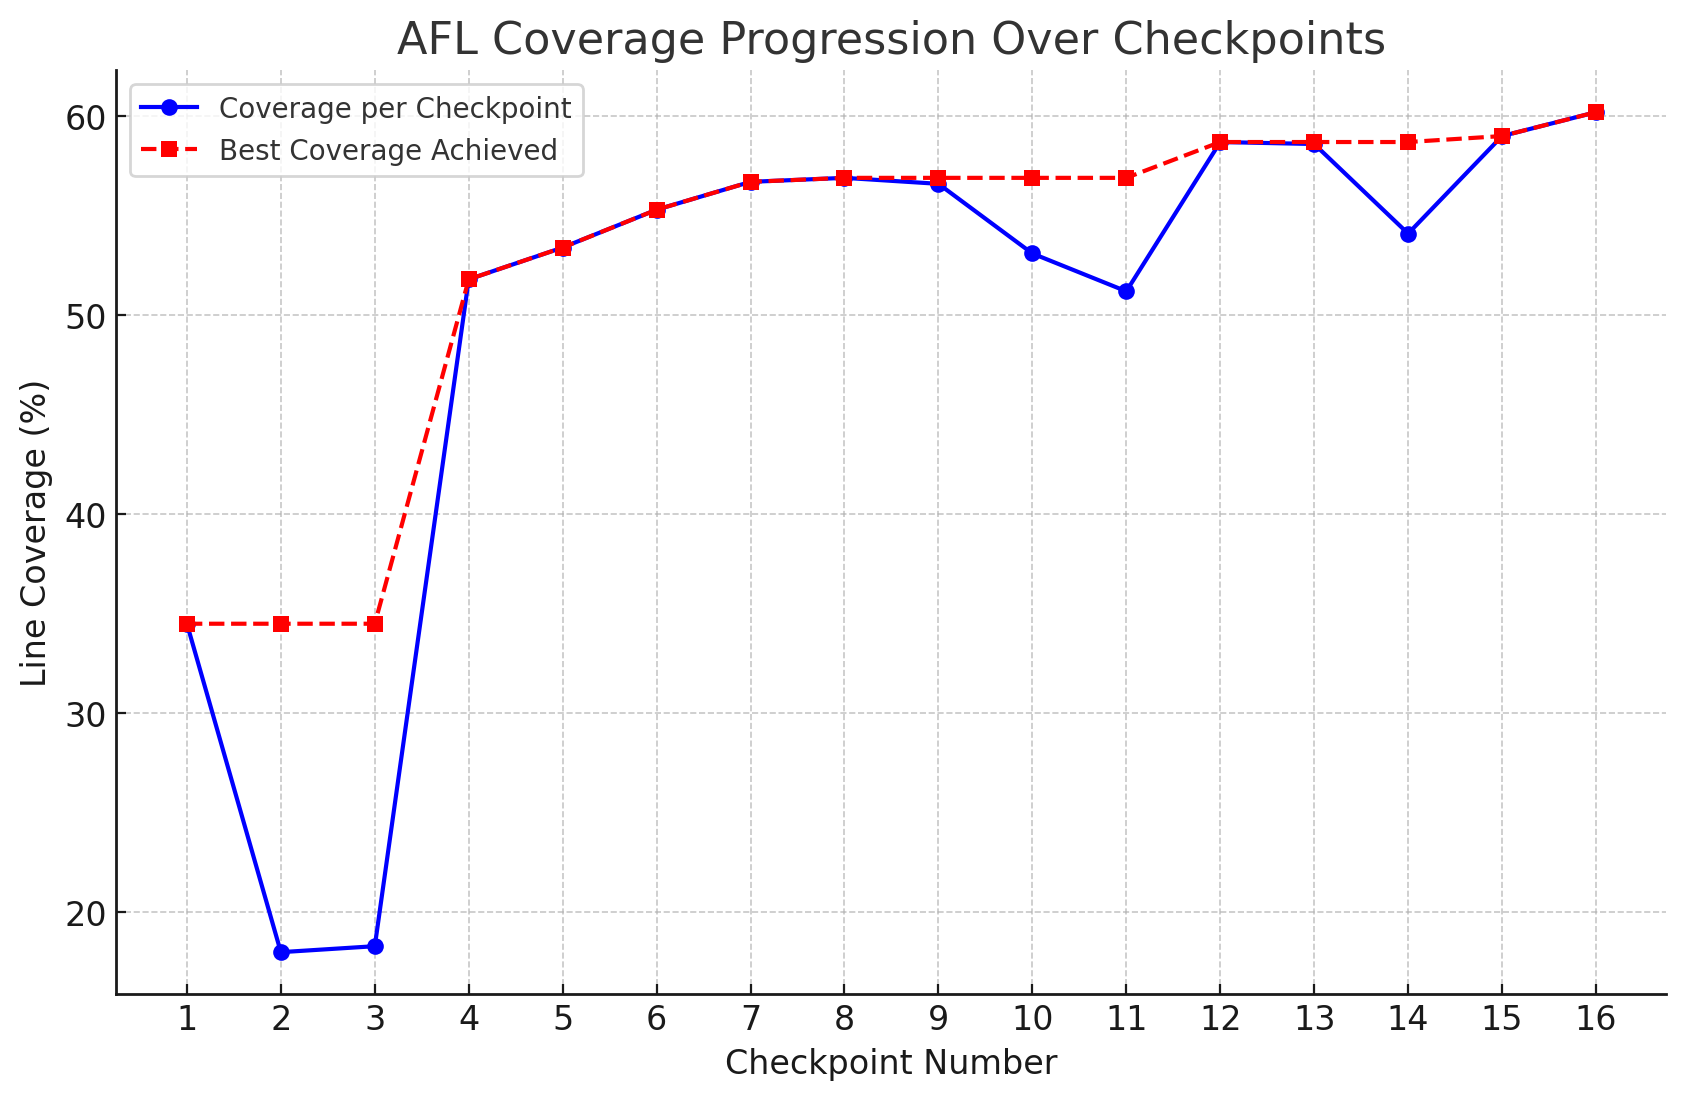
\includegraphics[width=0.5\textwidth]{AFL Coverage Progression Over Checkpoints.png}
    \caption{This Figure Shows the AFL Code Coverage Progression Over the 16 Checkpoints, Description of the strategies and methods used in each checkpoint can be found in the first section of the report.}
    \label{fig:coverage}
\end{figure}

\begin{figure}
    \centering
    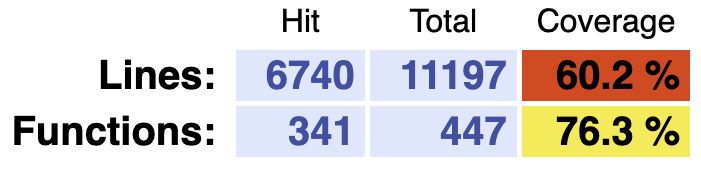
\includegraphics[width=0.5\textwidth]{Final Code Coverage.png}
    \caption{This Figure Shows the Final Line and Function Coverage of the AFL Fuzzer after the 16 Checkpoints.}
    \label{fig:final}
\end{figure}

\section{Failures and Potential Issues}
During the fuzzing process, several failures were encountered. One common issue arose when the compiler command string supplied to AFL was not structured correctly. Some compiler options caused TCC to fail immediately, which led to AFL generating useless test cases that did not contribute to coverage. This issue highlights the importance of carefully crafting the fuzzer execution string to ensure that meaningful test cases are executed rather than causing early failures.

Another issue involved timeouts, where certain mutated test cases took too long to compile, causing AFL to terminate them. This might have occurred when complex or syntactically incorrect inputs led to excessive loops or recursion within the compiler. These timeouts reduced the effectiveness of the fuzzer, as they prevented certain execution paths from being fully explored.

In terms of theoretical failures, one possible issue is crashes due to unhandled compiler bugs. Since AFL generates inputs that may expose edge cases, it is possible that certain mutations could trigger segmentation faults, infinite loops, or memory corruption errors. Additionally, incorrect handling of preprocessor directives or inline assembly could lead to unexpected behavior, such as failing to parse valid input or producing incorrect assembly output. These types of failures would indicate deeper issues within the TCC compiler's implementation and would need further debugging and validation.

Another potential failure is incorrect code generation, where the compiler produces faulty machine code due to mishandled edge cases in the optimization or code generation phase. This could lead to unexpected runtime behavior, where compiled programs crash or produce incorrect results even if they compile successfully.

One more theoretical failure involves resource exhaustion, where AFL generates input that causes excessive memory allocation or CPU usage, leading to a denial-of-service condition. This could be due to deep recursion, large unoptimized loops, or excessive macro expansion in preprocessor-heavy test cases. If the compiler does not handle such cases properly, it may freeze or crash instead of just failing.

\section{Uncovered Functions in i386-asm.c, tccpp.c, and tcctools.c}

This section details some of the functions that were not covered during AFL fuzzing in the files \texttt{i386-asm.c}, \texttt{tccpp.c}, and \texttt{tcctools.c}, along with explanations for their lack of coverage and strategies to cover them.

\subsection{Uncovered Functions in i386-asm.c}

Several functions in \texttt{i386-asm.c} were not majorly covered during AFL fuzzing, primarily those related to low-level assembly processing, including register handling, memory displacement calculations, and opcode generation. These functions are listed below, since some of these files have many uncovered functions, we will only list the ones that are not majorly covered:

\begin{verbatim}
get_reg_shift | asm_parse_numeric_reg | 
gen_expr64 | gen_disp32 | asm_modrm |
maybe_print_stats | asm_parse_regvar
\end{verbatim}

These functions were not covered due to the lack of seed programs using complex inline assembly constructs, such as explicit register shifts, numeric register parsing, memory displacement operations, and dynamic instruction modifications.

\subsubsection{Strategies to Cover These Functions}

To improve coverage, test cases with extensive inline assembly should be introduced, including direct register manipulations and displacement-based memory accesses. Adding seed programs that leverage assembly-based arithmetic operations, instruction encoding, and opcode modifications will also be beneficial. Additionally, ensuring that fuzzer-generated inputs include variations in instruction formatting and different operand addressing modes can help explore untested paths. Incorporating tests that utilize 64-bit expressions and function calls that interact with opcode parsing and execution logic will further increase coverage and ensure these functions are exercised during fuzzing.

\subsection{Uncovered Functions in tccpp.c}

Several functions in \texttt{tccpp.c} were not covered during AFL fuzzing, primarily those related to preprocessing operations, token manipulation, and macro handling. These functions are listed below:

\begin{verbatim}
cstr_reset | label_pop | tok_print | 
pp_debug_defines | pp_check_he0xE
\end{verbatim}

These functions were not covered due to the lack of test cases focusing on advanced preprocessing behaviors, such as handling complex macro definitions, token debugging, and preprocessor conditionals. The absence of test cases specifically designed to interact with preprocessing logic resulted in these functions remaining unexecuted.

\subsubsection{Strategies to Cover These Functions}

To improve coverage, test cases that rely heavily on preprocessor directives should be introduced, including complex macro definitions, conditional compilation, and token manipulation. Adding test cases that simulate real-world preprocessing scenarios, such as handling deeply nested macros, token pasting, and multi-line macro expansions, can help ensure execution of these functions. Additionally, enabling debugging features within the preprocessor and feeding inputs that interact with macro expansion and token reformatting will further improve coverage.

\subsection{Uncovered Functions in tcctools.c}

The following functions in \texttt{tcctools.c} were not covered during the fuzzing process:

\begin{verbatim}
le2belong | ar_usage | tcc_tool_cross 
gen_makedeps
\end{verbatim}

These functions primarily deal with byte-order conversion, error reporting for archive usage, cross-compilation execution, and dependency file generation. The lack of coverage suggests that the fuzzer did not generate inputs that exercised these functionalities, possibly due to missing execution paths leading to these functions.

\subsubsection{Strategies to Cover These Functions}

To cover these functions, specific test cases should be introduced that trigger library creation (using the `tcc -ar` flag), dependency generation (using the `tcc -M` flag), and cross-compilation processes. Additionally, ensuring that the fuzzer explores different command-line arguments that invoke these functionalities would be an effective strategy for improving coverage in \texttt{tcctools.c}. Introducing seed files that require cross-compilation or dependency tracking may also help improve the coverage.
% \begin{thebibliography}{00}
% \end{thebibliography}

\vspace{12pt}
\textit{This homework and report are completed with the help of resources provided along with the homework. This report makes use of GPT-4o to refine the content.}

\end{document}
